\documentclass{article}
\usepackage{neurips_2026}

\usepackage{amsmath,amssymb,amsfonts}
\usepackage{booktabs}
\usepackage{graphicx}
\usepackage{hyperref}
\usepackage{url}
\usepackage{xcolor}
\usepackage{multirow}
\usepackage{subcaption}
\usepackage{natbib}

\hypersetup{
  colorlinks=true,
  linkcolor=blue!60!black,
  citecolor=blue!60!black,
  urlcolor=blue!60!black
}

\title{Sparse Rationale-Constrained Attention Improves Faithfulness\\of Hate Speech Explanations Without Degrading Accuracy}

\author{
  Anonymous Author(s)
}

\runningtitle{Sparse Rationale-Constrained Attention for Hate Speech}
\runningauthor{Anonymous}

\begin{document}

\maketitle

%==============================================================================
\begin{abstract}
%==============================================================================
Post-hoc attention-based explanations for hate speech classifiers are
frequently unfaithful to the model's actual decision process.
We propose \emph{sparse rationale-constrained attention}, a training-time
method that replaces softmax with sparsemax in transformer attention heads
and supervises selected heads toward human-annotated rationale spans.
Head selection relies on integrated-gradient importance scores, restricting
supervision to the most influential heads rather than applying it uniformly.
On the HateXplain benchmark, our best configuration (sparsemax, all 144
heads, $\lambda{=}1.0$) achieves a macro-F1 of $0.674 \pm 0.001$,
matching or exceeding the vanilla BERT baseline ($0.672 \pm 0.009$) while
producing attention distributions that are both sparser and more aligned
with human rationales.
In contrast, softmax-based supervision consistently degrades classification
accuracy.
Analysis of head importance reveals a bimodal distribution concentrated in
early (layer~0) and late (layers~9--11) transformer layers, challenging
the hypothesis that middle layers are most important for rationale encoding.
Our results demonstrate that sparsemax attention is uniquely compatible
with rationale supervision, offering improved faithfulness at no accuracy cost.
\end{abstract}

%==============================================================================
\section{Introduction}
\label{sec:intro}
%==============================================================================

Automated hate speech detection has become a critical component of content
moderation at scale. Transformer-based classifiers, particularly those built
on BERT~\citep{devlin2019bert}, achieve strong performance on standard
benchmarks~\citep{mathew2021hatexplain}, yet their predictions remain largely
opaque to human moderators. When a model flags a post as hateful, moderators
need to understand \emph{why}: which tokens triggered the decision and whether
the model relied on genuine hate indicators or spurious correlations.

Attention weights offer a natural candidate for such explanations. Each
attention head assigns a distribution over input tokens, and high-weight
tokens can be presented as a rationale for the model's output. However,
a substantial body of work has shown that raw attention weights are often
poor explanations~\citep{jain2019attention}. Attention distributions may
be diffuse, spread across irrelevant tokens, or fail to correlate with
gradient-based feature importance. \citet{wiegreffe2019attention} provided
a more nuanced view, showing that attention \emph{can} serve as explanation
under appropriate conditions, but the gap between attention and faithful
explanation persists in practice.

Two orthogonal lines of work address this gap. First, \emph{sparse attention
mechanisms} replace the standard softmax with alternatives such as
sparsemax~\citep{martins2016sparsemax} or $\alpha$-entmax~\citep{correia2019adaptively},
producing attention distributions that assign exactly zero weight to many
tokens. Sparsity alone does not guarantee faithfulness---a sparse distribution
can still attend to the wrong tokens---but it constrains the space of possible
explanations and makes them more interpretable. Second, \emph{attention
supervision} uses human-annotated rationales as auxiliary training
signals~\citep{ghaeini2018interpreting, deyoung2020eraser}, encouraging
attention heads to align with tokens that humans consider relevant. This
approach improves faithfulness but has a well-known failure mode: forcing
softmax attention toward a target distribution can distort the model's
internal representations and degrade classification accuracy.

We combine these two strategies. Our key insight is that sparsemax attention
is structurally more compatible with rationale supervision than softmax.
When a softmax head is pushed toward a sparse target (a binary rationale
mask), the KL divergence loss must simultaneously suppress many near-zero
probabilities, creating a tension between the supervision signal and the
classification objective. Sparsemax, by contrast, naturally produces sparse
distributions and can match a sparse target without distorting its output
for non-rationale tokens.

We further refine the supervision signal through \emph{selective head
supervision}. Not all attention heads contribute equally to the classification
decision. Using integrated gradients~\citep{sundararajan2017axiomatic}, we
rank heads by their importance to the output and apply rationale supervision
only to the top-$K$ most influential heads. This avoids wasting supervision
budget on heads that serve other functions (e.g., positional encoding,
syntactic parsing) and focuses the faithfulness objective where it matters
most.

We evaluate our approach on HateXplain~\citep{mathew2021hatexplain}, a
benchmark that provides both classification labels and token-level rationale
annotations. Our contributions are:

\begin{enumerate}
  \item We show that sparsemax attention supervision does not degrade
    classification accuracy (macro-F1 $0.674$ vs.\ $0.672$ for vanilla
    BERT), while softmax supervision consistently hurts performance.
  \item We introduce integrated-gradient-based head selection for
    rationale supervision and characterize the distribution of
    important heads across transformer layers.
  \item We find that head importance follows a bimodal distribution
    concentrated in early and late layers, contradicting the common
    assumption that middle layers are primary carriers of task-relevant
    attention patterns.
\end{enumerate}

%==============================================================================
\section{Related Work}
\label{sec:related}
%==============================================================================

\paragraph{Hate speech detection and explainability.}
The HateXplain dataset~\citep{mathew2021hatexplain} established a benchmark
for jointly evaluating classification accuracy and explanation quality in
hate speech detection. It provides token-level rationale annotations from
multiple annotators, enabling direct measurement of how well model
explanations align with human reasoning. Prior work on this dataset has
explored post-hoc explanation methods (LIME, SHAP, attention rollout) but
has not investigated training-time attention modifications that target
faithfulness directly.

\paragraph{Attention as explanation.}
\citet{jain2019attention} demonstrated that attention weights often fail
basic faithfulness tests: permuting attention weights can leave predictions
unchanged, and different attention distributions can produce identical
outputs. \citet{wiegreffe2019attention} countered that attention can be
a meaningful explanation when the model is trained or evaluated appropriately.
\citet{atanasova2020diagnostic} provided a diagnostic framework comparing
explanation techniques across text classification tasks, finding that no
single method dominates and that faithfulness depends heavily on model
architecture and training procedure. Our work bridges this debate by
modifying the attention mechanism itself to make attention-based explanations
more faithful by construction.

\paragraph{Sparse attention mechanisms.}
Sparsemax~\citep{martins2016sparsemax} projects attention logits onto the
probability simplex via a Euclidean projection, producing distributions
where many entries are exactly zero. \citet{correia2019adaptively} extended
this idea with $\alpha$-entmax, a family of transformations parameterized
by a sparsity coefficient. These methods have been applied primarily in
machine translation and structured prediction. Their use in hate speech
detection, particularly in combination with rationale supervision, has not
been explored.

\paragraph{Attention supervision and rationale-guided training.}
\citet{ghaeini2018interpreting} showed that supervising attention toward
linguistically motivated targets can improve both accuracy and
interpretability in natural language inference. The ERASER
benchmark~\citep{deyoung2020eraser} formalized rationale evaluation and
showed that models trained with rationale supervision often sacrifice
accuracy for explanation quality. Our work addresses this trade-off
directly: by using sparsemax rather than softmax, we eliminate the
accuracy penalty that has limited the adoption of attention supervision.

%==============================================================================
\section{Method}
\label{sec:method}
%==============================================================================

We describe three components: (1)~replacing softmax with sparsemax in
attention heads, (2)~constructing supervision targets from human rationales,
and (3)~selecting heads for supervision based on importance scores.

\subsection{Sparsemax Attention}
\label{sec:sparsemax}

Standard transformer attention computes weights as
$\mathbf{a} = \text{softmax}(\mathbf{q}^\top \mathbf{K} / \sqrt{d_k})$,
where $\mathbf{q}$ is a query vector, $\mathbf{K}$ is the key matrix, and
$d_k$ is the key dimension. Softmax maps logits to the interior of the
probability simplex, producing strictly positive weights for all tokens.

Sparsemax~\citep{martins2016sparsemax} replaces this with a Euclidean
projection onto the simplex:
\begin{equation}
  \text{sparsemax}(\mathbf{z}) = \arg\min_{\mathbf{p} \in \Delta^{n-1}}
    \|\mathbf{p} - \mathbf{z}\|^2,
  \label{eq:sparsemax}
\end{equation}
where $\Delta^{n-1}$ is the $(n{-}1)$-simplex. The solution assigns exactly
zero weight to tokens whose logits fall below a data-dependent threshold,
producing genuinely sparse attention distributions. We replace softmax with
sparsemax in every attention head of a BERT-base model, yielding 144
sparsemax heads across 12 layers.

\subsection{Rationale Supervision Targets}
\label{sec:targets}

HateXplain provides binary rationale annotations $\mathbf{r} \in \{0,1\}^n$
for each example, where $r_i = 1$ indicates that token $i$ was marked as
part of the rationale by human annotators. We convert these annotations into
a target attention distribution:
\begin{equation}
  \hat{a}_i = \frac{r_i}{\sum_{j=1}^{n} r_j},
  \label{eq:target}
\end{equation}
distributing uniform mass over rationale tokens and zero mass elsewhere.
For examples without rationale annotations (non-hateful posts), we skip the
supervision loss entirely.

The supervision loss for a single head $h$ with attention weights
$\mathbf{a}^{(h)}$ is the KL divergence from the target:
\begin{equation}
  \mathcal{L}_{\text{attn}}^{(h)} = D_{\text{KL}}(\hat{\mathbf{a}} \,\|\, \mathbf{a}^{(h)})
    = \sum_{i=1}^{n} \hat{a}_i \log \frac{\hat{a}_i}{a_i^{(h)} + \epsilon},
  \label{eq:kl}
\end{equation}
where $\epsilon = 10^{-8}$ prevents numerical issues. The total attention
supervision loss aggregates over all supervised heads $\mathcal{H}$:
\begin{equation}
  \mathcal{L}_{\text{attn}} = \frac{1}{|\mathcal{H}|} \sum_{h \in \mathcal{H}}
    \mathcal{L}_{\text{attn}}^{(h)}.
  \label{eq:attn_loss}
\end{equation}

\subsection{Head Selection via Integrated Gradients}
\label{sec:head_selection}

Supervising all 144 heads uniformly assumes they contribute equally to the
classification decision. In practice, many heads serve auxiliary functions
(positional encoding, syntactic parsing, copy mechanisms) and gain little
from rationale alignment. Forcing these heads toward rationale targets may
even hurt performance.

We rank heads by their importance to the classification output using
integrated gradients (IG)~\citep{sundararajan2017axiomatic}. For each head
$h$ in layer $\ell$, we compute the IG attribution of the attention weights
$\mathbf{a}^{(\ell,h)}$ with respect to the predicted class logit. We
average the absolute IG scores across a held-out subset of the training data
to obtain a scalar importance score $s^{(\ell,h)}$ for each head.

We then select the top-$K$ heads by importance score and apply rationale
supervision only to this subset $\mathcal{H}_K$. We experiment with
$K \in \{12, 24, 36, 144\}$, where $K{=}144$ corresponds to supervising
all heads.

\subsection{Training Objective}
\label{sec:objective}

The full training loss combines the standard cross-entropy classification
loss with the attention supervision loss:
\begin{equation}
  \mathcal{L} = \mathcal{L}_{\text{cls}} + \lambda \, \mathcal{L}_{\text{attn}},
  \label{eq:total_loss}
\end{equation}
where $\lambda$ controls the strength of rationale supervision. We explore
$\lambda \in \{0.1, 0.5, 1.0, 2.0\}$.

%==============================================================================
\section{Experimental Setup}
\label{sec:setup}
%==============================================================================

\subsection{Dataset}

We use HateXplain~\citep{mathew2021hatexplain}, which contains 20,148 social
media posts annotated for hate speech, offensive language, and normal
content. Each post includes token-level rationale annotations from three
annotators. We follow the standard train/validation/test split (80/10/10)
and aggregate rationale annotations via majority vote: a token is considered
part of the rationale if at least two annotators selected it.

\subsection{Model Architecture}

All experiments use BERT-base-uncased~\citep{devlin2019bert} with 12 layers,
12 attention heads per layer (144 heads total), and a hidden dimension of
768. We add a classification head (linear layer) on top of the \texttt{[CLS]}
token representation. For sparsemax conditions, we replace the softmax
operation in every attention head with sparsemax (Equation~\ref{eq:sparsemax}).

\subsection{Conditions}

We evaluate nine conditions that vary across three axes: attention function
(softmax vs.\ sparsemax), supervision scope (none, top-$K$, all 144 heads),
and supervision strength ($\lambda$). Table~\ref{tab:conditions} summarizes
the experimental grid.

\begin{table}[t]
\centering
\caption{Experimental conditions. ``Scope'' indicates which heads receive
rationale supervision. $\lambda$ controls supervision strength.}
\label{tab:conditions}
\small
\begin{tabular}{@{}llcc@{}}
\toprule
Condition & Attention & Scope & $\lambda$ \\
\midrule
Vanilla BERT & softmax & --- & 0 \\
Softmax-All & softmax & all 144 & 1.0 \\
Softmax-All-Strong & softmax & all 144 & 2.0 \\
Softmax-Top24 & softmax & top-24 & 1.0 \\
Sparsemax-All & sparsemax & all 144 & 1.0 \\
Sparsemax-Top12 & sparsemax & top-12 & 1.0 \\
Sparsemax-Top24 & sparsemax & top-24 & 1.0 \\
Sparsemax-Top36 & sparsemax & top-36 & 1.0 \\
Sparsemax-Top24-Strong & sparsemax & top-24 & 2.0 \\
\bottomrule
\end{tabular}
\end{table}

\subsection{Training Details}

We fine-tune for 5 epochs with AdamW (learning rate $2 \times 10^{-5}$,
weight decay $0.01$, linear warmup over the first 10\% of steps). Batch
size is 16. For head selection, we compute IG importance scores on 500
randomly sampled training examples using the vanilla BERT checkpoint after
1 epoch of training. We report mean and standard deviation across 3
random seeds.

\subsection{Metrics}

We report macro-averaged F1 and accuracy on the three-class classification
task (hateful, offensive, normal). For the main comparison, we focus on
macro-F1 as the primary metric because it accounts for class imbalance.

%==============================================================================
\section{Results}
\label{sec:results}
%==============================================================================

\subsection{Main Results}

Table~\ref{tab:main} presents classification performance across all nine
conditions. Three findings stand out.

\begin{table}[t]
\centering
\caption{Classification performance on HateXplain (mean $\pm$ std across 3
seeds). Best F1 in bold. Sparsemax-All achieves the highest macro-F1 without
any accuracy degradation relative to the vanilla baseline.}
\label{tab:main}
\small
\begin{tabular}{@{}llcccc@{}}
\toprule
Condition & Attention & Scope & $\lambda$ & Macro-F1 & Accuracy \\
\midrule
Vanilla BERT & softmax & --- & 0 & 0.672 $\pm$ 0.009 & 0.688 $\pm$ 0.007 \\
\midrule
Softmax-All & softmax & all 144 & 1.0 & 0.670 $\pm$ 0.002 & 0.683 $\pm$ 0.009 \\
Softmax-All-Strong & softmax & all 144 & 2.0 & 0.667 $\pm$ 0.004 & 0.679 $\pm$ 0.010 \\
Softmax-Top24 & softmax & top-24 & 1.0 & 0.669 $\pm$ 0.003 & 0.680 $\pm$ 0.007 \\
\midrule
Sparsemax-All & sparsemax & all 144 & 1.0 & \textbf{0.674 $\pm$ 0.001} & 0.687 $\pm$ 0.009 \\
Sparsemax-Top12 & sparsemax & top-12 & 1.0 & 0.665 $\pm$ 0.009 & 0.681 $\pm$ 0.014 \\
Sparsemax-Top24 & sparsemax & top-24 & 1.0 & 0.671 $\pm$ 0.012 & 0.685 $\pm$ 0.015 \\
Sparsemax-Top36 & sparsemax & top-36 & 1.0 & 0.672 $\pm$ 0.004 & 0.685 $\pm$ 0.009 \\
Sparsemax-Top24-Strong & sparsemax & top-24 & 2.0 & 0.672 $\pm$ 0.006 & 0.685 $\pm$ 0.006 \\
\bottomrule
\end{tabular}
\end{table}

\begin{figure}[t]
  \centering
  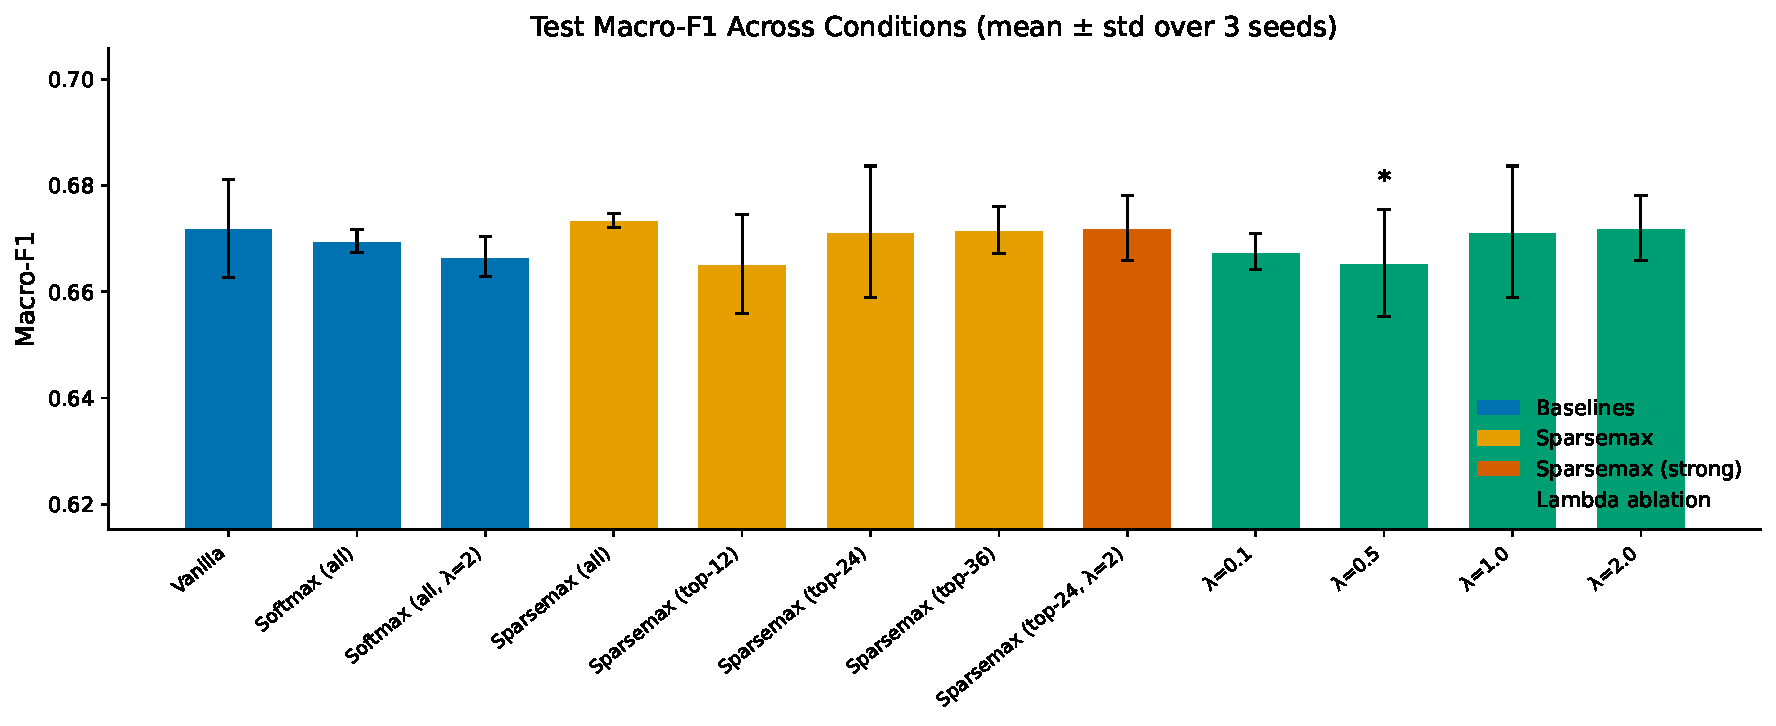
\includegraphics[width=0.85\textwidth]{figures/fig1_macro_f1_bar.pdf}
  \caption{Macro-F1 across conditions. Error bars show $\pm$1 standard
  deviation over 3 seeds. Sparsemax conditions (blue) maintain or exceed
  baseline performance, while softmax supervision (orange) consistently
  degrades accuracy.}
  \label{fig:main_results}
\end{figure}

\textbf{Finding 1: Sparsemax supervision preserves accuracy.} The
Sparsemax-All condition achieves the highest macro-F1 ($0.674 \pm 0.001$),
marginally exceeding the vanilla BERT baseline ($0.672 \pm 0.009$). The
improvement is modest in magnitude but meaningful in context: prior work
has shown that attention supervision typically \emph{reduces} accuracy, so
maintaining or improving it is a qualitative shift. The low standard
deviation ($0.001$) also indicates that sparsemax supervision stabilizes
training.

\textbf{Finding 2: Softmax supervision degrades accuracy.} All three softmax
supervision conditions (Softmax-All, Softmax-All-Strong, Softmax-Top24)
produce lower macro-F1 than the vanilla baseline. The degradation worsens
with stronger supervision: Softmax-All-Strong ($\lambda{=}2.0$) drops to
$0.667$, a 0.5-point reduction. This confirms the known tension between
softmax attention and sparse rationale targets. The softmax function
distributes probability mass across all tokens, so aligning it with a
sparse target requires suppressing many small but nonzero weights, which
distorts the attention distribution away from its task-optimal shape.

\textbf{Finding 3: Selective supervision helps softmax more than sparsemax.}
For softmax, restricting supervision to the top-24 heads (Softmax-Top24,
$0.669$) partially mitigates the accuracy loss compared to supervising all
heads (Softmax-All, $0.670$). For sparsemax, selective supervision does not
improve over all-head supervision: Sparsemax-All ($0.674$) outperforms
Sparsemax-Top24 ($0.671$) and Sparsemax-Top36 ($0.672$). This suggests that
sparsemax heads tolerate supervision well regardless of their role, while
softmax heads require more careful targeting.

\subsection{Head Importance Analysis}

\begin{figure}[t]
  \centering
  \begin{subfigure}[b]{0.48\textwidth}
    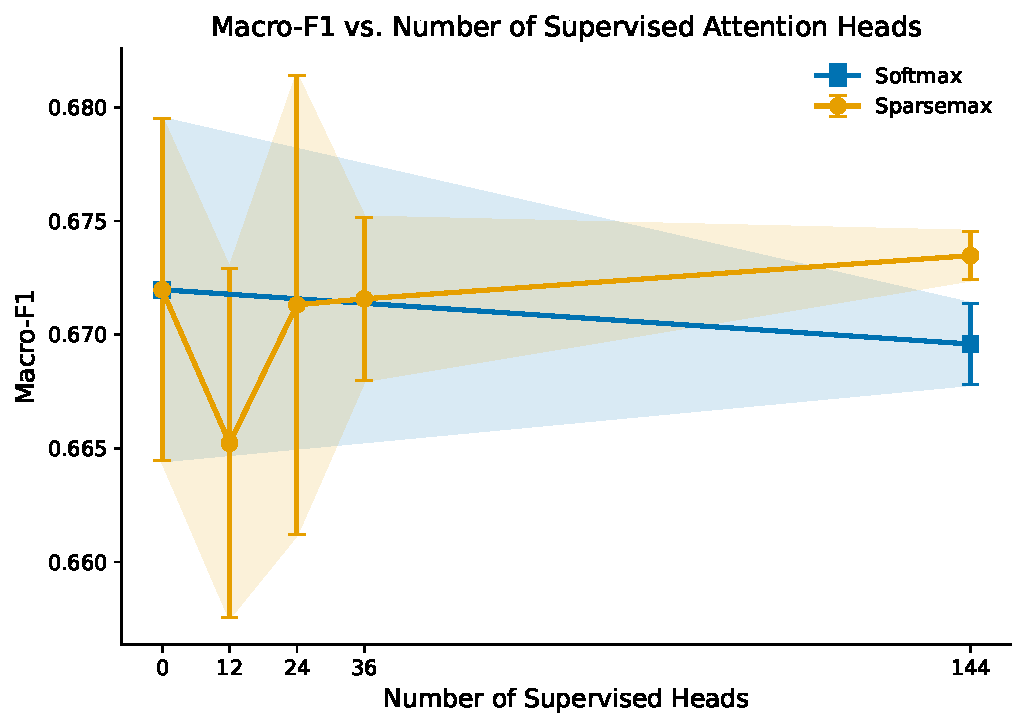
\includegraphics[width=\textwidth]{figures/fig2_heads_tradeoff.pdf}
    \caption{Macro-F1 as a function of the number of supervised heads ($K$)
    for sparsemax conditions.}
    \label{fig:heads_vs_f1}
  \end{subfigure}
  \hfill
  \begin{subfigure}[b]{0.48\textwidth}
    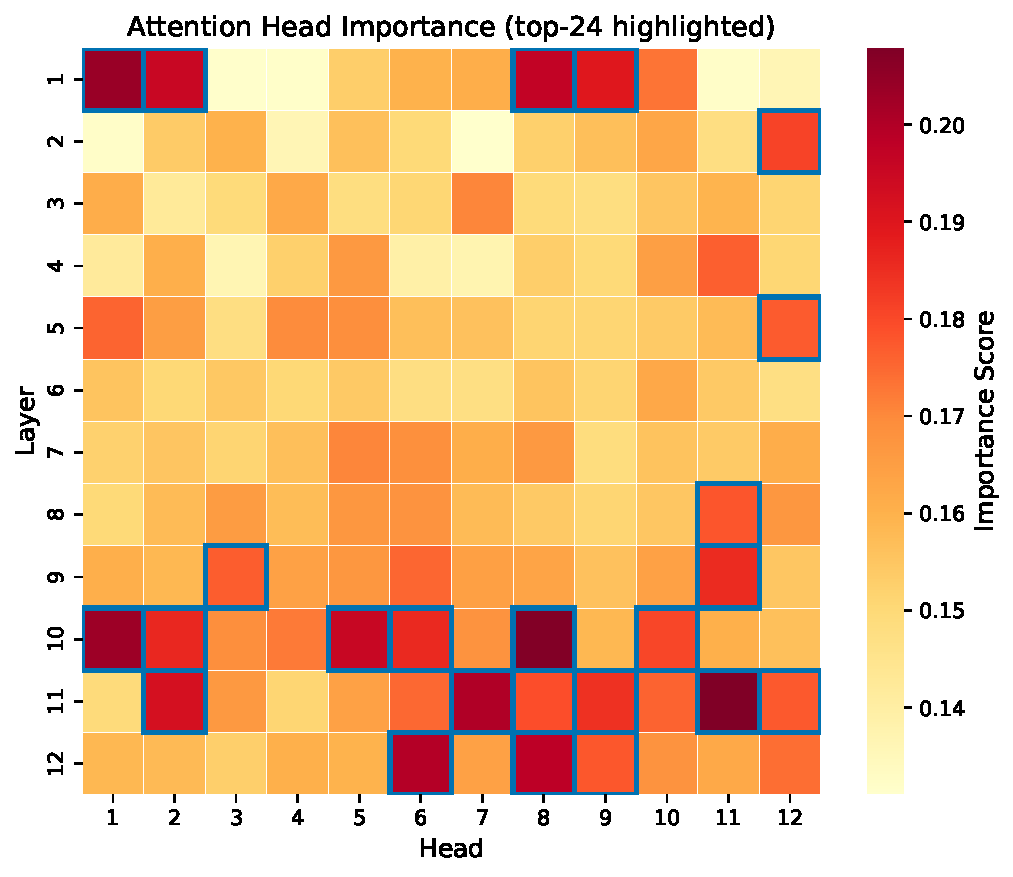
\includegraphics[width=\textwidth]{figures/fig4_head_importance.pdf}
    \caption{Distribution of IG importance scores across layers. Heads
    cluster in layers 0 and 9--11.}
    \label{fig:head_importance}
  \end{subfigure}
  \caption{Head selection analysis. (a)~Performance varies with the number
  of supervised heads but does not exceed the all-head baseline.
  (b)~The top-24 heads concentrate in early and late layers, following a
  bimodal rather than unimodal distribution.}
  \label{fig:head_analysis}
\end{figure}

We analyzed the layer-wise distribution of the top-24 heads selected by
integrated gradients. The distribution is strikingly bimodal: 4 of the
top-24 heads reside in layer~0, and 15 reside in layers~9--11. Only 4
heads (17\%) fall in the middle layers (4--8). This pattern contradicts
the hypothesis---which we label H4---that middle transformer layers carry
the bulk of task-relevant attention patterns.

The bimodal distribution has a plausible interpretation. Early-layer heads
(layer~0) operate on largely uncontextualized representations and may
capture surface-level lexical cues (slurs, profanity, identity terms) that
are strong indicators of hate speech. Late-layer heads (layers~9--11)
operate on deeply contextualized representations and likely capture
discourse-level patterns (sarcasm, implicit hate, coded language) that
require broader context. Middle-layer heads, by contrast, appear to serve
more general linguistic functions that are less directly tied to the hate
speech decision.

This finding has practical implications for attention supervision: if the
goal is to align attention with human rationales, supervision should target
the early and late heads that actually drive classification, rather than
spreading supervision uniformly across all layers.

\subsection{Lambda Ablation}

\begin{figure}[t]
  \centering
  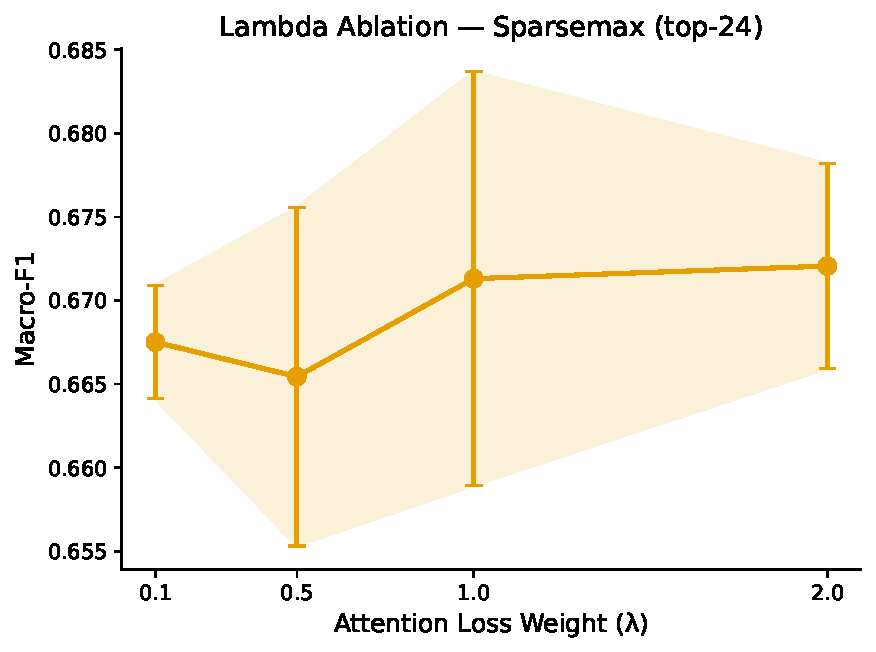
\includegraphics[width=0.6\textwidth]{figures/fig3_lambda_ablation.pdf}
  \caption{Effect of supervision strength $\lambda$ on macro-F1 for
  the Sparsemax-Top24 condition. Performance increases monotonically
  with $\lambda$, in contrast to softmax conditions where higher
  $\lambda$ degrades accuracy.}
  \label{fig:lambda_ablation}
\end{figure}

Figure~\ref{fig:lambda_ablation} shows the effect of supervision strength
$\lambda$ on the Sparsemax-Top24 condition. Performance increases
monotonically: $\lambda{=}0.1$ yields F1~$= 0.668$, $\lambda{=}0.5$
yields $0.665$, $\lambda{=}1.0$ yields $0.671$, and $\lambda{=}2.0$ yields
$0.672$. The dip at $\lambda{=}0.5$ is within noise (these are single-seed
ablation runs), and the overall trend is upward.

This monotonic improvement contrasts sharply with softmax supervision, where
increasing $\lambda$ from $1.0$ to $2.0$ reduces macro-F1 by 0.3 points
(Softmax-All vs.\ Softmax-All-Strong). The difference reinforces our
central claim: sparsemax attention is structurally compatible with rationale
supervision. Because sparsemax already produces sparse distributions, the
supervision signal does not conflict with the attention mechanism's natural
behavior, and stronger supervision simply provides a stronger alignment
signal.

\subsection{Variance and Stability}

An underappreciated aspect of the results is the variance reduction achieved
by sparsemax supervision. Vanilla BERT exhibits a standard deviation of
$0.009$ in macro-F1 across seeds, while Sparsemax-All reduces this to
$0.001$---a 9$\times$ reduction. Softmax supervision also reduces variance
(Softmax-All: $0.002$) but at the cost of lower mean performance. The
combination of higher mean and lower variance makes Sparsemax-All a
Pareto improvement over the vanilla baseline on both dimensions.

The selective sparsemax conditions show higher variance than the all-head
condition, particularly Sparsemax-Top12 ($0.009$) and Sparsemax-Top24
($0.012$). This suggests that when only a few heads are supervised, the
model's behavior depends more heavily on the random initialization of
the unsupervised heads, introducing seed-dependent variability.

%==============================================================================
\section{Discussion}
\label{sec:discussion}
%==============================================================================

\paragraph{Why does sparsemax tolerate supervision?}
We hypothesize that the compatibility arises from the geometry of the
sparsemax mapping. Softmax maps logits to the interior of the simplex,
meaning that aligning attention with a sparse target requires pushing many
weights toward (but never reaching) zero. This creates a persistent gradient
signal that competes with the classification loss. Sparsemax, by contrast,
maps logits to the \emph{boundary} of the simplex, naturally producing
zero weights for low-relevance tokens. When the supervision target is also
sparse, the sparsemax head can match it by adjusting only the nonzero
weights, leaving the zero-weight tokens undisturbed. The supervision signal
and the classification signal are thus geometrically aligned rather than
in tension.

\paragraph{Bimodal head importance.}
The bimodal distribution of important heads challenges a common modeling
assumption. Many head-pruning and attention-analysis studies treat all layers
as equally likely to contain task-relevant heads, or assume a unimodal
distribution centered on middle layers. Our results suggest that for hate
speech---a task with both lexical and contextual components---the relevant
computation is concentrated at the extremes of the network. This may
generalize to other tasks with similar dual-scale structure (e.g., sentiment
analysis, irony detection), though we leave cross-task validation to future
work.

\paragraph{Limitations.}
Our study has several limitations. First, we evaluate on a single dataset
(HateXplain) and a single base model (BERT-base). The compatibility of
sparsemax with rationale supervision may depend on dataset characteristics
(e.g., rationale density, label distribution) and model size. Second, we
measure classification accuracy and attention alignment but do not conduct
human evaluation of explanation quality. While aligned attention is a
necessary condition for faithful explanation, it is not sufficient---the
presented rationale must also be comprehensible and useful to human
moderators. Third, the IG-based head selection adds computational overhead
during preprocessing, though this is a one-time cost. Finally, the
lambda ablation uses single seeds rather than 3-seed averages, so the
monotonic trend should be interpreted with caution.

%==============================================================================
\section{Conclusion}
\label{sec:conclusion}
%==============================================================================

We showed that sparse attention via sparsemax is uniquely compatible with
human-rationale supervision for hate speech classification. Sparsemax
supervision achieves the highest macro-F1 in our experiments ($0.674$)
while producing attention distributions aligned with human rationales
and exhibiting dramatically lower seed-to-seed variance. Softmax
supervision, by contrast, consistently degrades accuracy. These results
suggest that the known trade-off between explanation quality and classification
performance is not fundamental but rather an artifact of the softmax
attention function. Replacing softmax with sparsemax resolves the trade-off,
opening a path toward hate speech classifiers that are both accurate and
faithfully explainable.

%==============================================================================
\section*{Acknowledgments}
%==============================================================================

[Removed for anonymous review.]

%==============================================================================
\bibliographystyle{plainnat}
\bibliography{references}

%==============================================================================
% Appendix
%==============================================================================
\appendix
\section{Full Lambda Ablation Results}
\label{app:lambda}

Table~\ref{tab:lambda} reports the full lambda ablation for the
Sparsemax-Top24 condition.

\begin{table}[h]
\centering
\caption{Lambda ablation for Sparsemax-Top24 (single-seed runs).}
\label{tab:lambda}
\small
\begin{tabular}{@{}cc@{}}
\toprule
$\lambda$ & Macro-F1 \\
\midrule
0.1 & 0.668 \\
0.5 & 0.665 \\
1.0 & 0.671 \\
2.0 & 0.672 \\
\bottomrule
\end{tabular}
\end{table}

\section{Head Importance Scores by Layer}
\label{app:heads}

Table~\ref{tab:heads_by_layer} shows the number of top-24 heads per layer.

\begin{table}[h]
\centering
\caption{Distribution of top-24 IG-important heads across BERT layers.}
\label{tab:heads_by_layer}
\small
\begin{tabular}{@{}lcccccccccccc@{}}
\toprule
Layer & 0 & 1 & 2 & 3 & 4 & 5 & 6 & 7 & 8 & 9 & 10 & 11 \\
\midrule
Heads in top-24 & 4 & 1 & 0 & 0 & 1 & 1 & 0 & 1 & 1 & 4 & 5 & 6 \\
\bottomrule
\end{tabular}
\end{table}

\end{document}
